% =========================================================================
% BÀI 37: LUYỆN TẬP CHUNG (CHỦ ĐỀ 9: THỜI GIAN. GIỜ VÀ LỊCH)
% TOÀN BỘ CÂU HỎI ĐƯỢC VẼ HÌNH MINH HỌA TRỰC QUAN 100% BẰNG TIKZ 2D
% =========================================================================

% --- ĐỊNH NGHĨA MÀU SẮC AN TOÀN ---
\colorlet{myteal}{cyan!70!blue}
\colorlet{myorange}{orange}
\colorlet{mypurple}{purple}
\colorlet{myblue}{blue}
\colorlet{myred}{red}

% --- CÁC HÀM VẼ HÌNH TRỰC QUAN ĐẶC TRƯNG CHO BÀI 37 ---

% 1. Vẽ đồng hồ kim (mặt tròn có chân đế và kim chỉ giờ)
\providecommand{\VeDongHoKim}[4]{% #1=scale, #2=(x,y), #3=gio, #4=mau
  \begin{scope}[shift={(#2)}, scale=#1]
    \draw[line width=1.3pt, #4!80] (-0.45,-0.92) -- (-0.72,-1.18);
    \draw[line width=1.3pt, #4!80] (0.45,-0.92) -- (0.72,-1.18);
    \draw[fill=#4!12, draw=#4!85, line width=1.1pt] (0,0) circle (1.14cm);
    \draw[fill=white, draw=black!60, line width=0.6pt] (0,0) circle (0.98cm);
    \foreach \n in {1,...,12} {
      \pgfmathsetmacro{\goc}{90 - \n * 30}
      \draw[line width=0.5pt, black!50] (\goc:0.88cm) -- (\goc:0.96cm);
      \node[font=\bfseries\tiny, color=black!90] at (\goc:0.75cm) {\n};
    }
    % Kim phút (chỉ số 12)
    \draw[line width=1.3pt, -{Latex[length=1.8mm, width=1.2mm]}, blue!85!black] (0,-0.06) -- (0,0.64);
    % Kim giờ (chỉ số #3)
    \pgfmathsetmacro{\gocht}{90 - #3 * 30}
    \draw[line width=1.9pt, -{Latex[length=2.0mm, width=1.6mm]}, red!85!black] (0,-0.04) -- (\gocht:0.45cm);
    \fill[orange!90!black, draw=black!80, line width=0.4pt] (0,0) circle (0.08cm);
  \end{scope}
}

% 2. Vẽ tờ lịch bóc tường / để bàn
\providecommand{\VeToLich}[4]{% #1=(x,y), #2=Thứ, #3=Số/Nội dung, #4=màu
  \begin{scope}[shift={(#1)}]
    \fill[black!70] (-0.45,0.65) circle (0.05cm);
    \fill[black!70] (0.45,0.65) circle (0.05cm);
    \draw[line width=1.0pt, black!50] (-0.45,0.65) -- (-0.45,0.8);
    \draw[line width=1.0pt, black!50] (0.45,0.65) -- (0.45,0.8);
    \draw[fill=white, draw=#4!85, line width=1.0pt, rounded corners=3pt] (-1.0,-0.65) rectangle (1.0,0.65);
    \draw[fill=#4!85, draw=#4!85, rounded corners=2pt] (-1.0,0.22) rectangle (1.0,0.65);
    \node[font=\bfseries\tiny, color=white] at (0,0.44) {#2};
    \node[font=\bfseries\scriptsize, color=#4!90!black] at (0,-0.2) {#3};
  \end{scope}
}

% 3. Đồng hồ điện tử để bàn
\providecommand{\VeDongHoDienTu}[3]{% #1=(x,y), #2=thời gian, #3=màu
  \begin{scope}[shift={(#1)}, scale=0.6]
    \draw[fill=#3!15, draw=#3!85, line width=0.9pt, rounded corners=3pt] (-1.3,-0.48) rectangle (1.3,0.48);
    \draw[fill=black!92, draw=black, rounded corners=2pt] (-1.12,-0.34) rectangle (1.12,0.34);
    \node[font=\bfseries\small, color=green!85!white] at (0,0) {#2};
  \end{scope}
}

% 4. Dải 7 ngày trong tuần
\providecommand{\VeDaiBayNgay}[2]{% #1=(x,y), #2=ngày nổi bật (1..7, 0 là không)
  \begin{scope}[shift={(#1)}, scale=0.56]
    \foreach \i/\thu/\mau in {1/{Thứ 2}/myblue, 2/{Thứ 3}/myblue, 3/{Thứ 4}/myblue, 4/{Thứ 5}/myblue, 5/{Thứ 6}/myblue, 6/{Thứ 7}/myorange, 7/{CN}/myred} {
      \pgfmathsetmacro{\x}{(\i-4)*1.95}
      \ifnum\i=#2
        \draw[fill=\mau!25, draw=\mau!90, line width=1.3pt, rounded corners=3pt] (\x-0.85,-0.52) rectangle (\x+0.85,0.52);
        \node[font=\bfseries\footnotesize, color=\mau!90!black] at (\x,0) {\thu};
        \node[above, font=\bfseries\tiny, color=red!85] at (\x,0.58) {$\blacktriangledown$};
      \else
        \draw[fill=white, draw=gray!70, line width=0.7pt, rounded corners=3pt] (\x-0.85,-0.52) rectangle (\x+0.85,0.52);
        \node[font=\bfseries\footnotesize, color=black!85] at (\x,0) {\thu};
      \fi
    }
  \end{scope}
}

% 5. Dải các ngày trong tuần kèm số ngày
\providecommand{\VeDaiTuanCoNgay}[2]{% #1=(x,y), #2=ngày bắt đầu
  \begin{scope}[shift={(#1)}, scale=0.55]
    \foreach \i/\thu/\mau in {0/{Thứ 2}/myblue, 1/{Thứ 3}/myblue, 2/{Thứ 4}/myblue, 3/{Thứ 5}/myblue, 4/{Thứ 6}/myblue, 5/{Thứ 7}/myorange, 6/{CN}/myred} {
      \pgfmathsetmacro{\x}{(\i-3)*1.95}
      \pgfmathtruncatemacro{\ngayso}{#2 + \i}
      \draw[fill=\mau!15, draw=\mau!85, line width=1.0pt, rounded corners=3pt] (\x-0.85,-0.65) rectangle (\x+0.85,0.65);
      \draw[fill=\mau!85, draw=\mau!85, rounded corners=2pt] (\x-0.85,0.2) rectangle (\x+0.85,0.65);
      \node[font=\bfseries\tiny, color=white] at (\x,0.43) {\thu};
      \node[font=\bfseries\small, color=\mau!90!black] at (\x,-0.2) {\ngayso};
    }
  \end{scope}
}

% =========================================================================
% BẮT ĐẦU NỘI DUNG 20 CÂU HỎI
% =========================================================================

\textbf{Phần 1. Trắc nghiệm lựa chọn}
\setcounterpageref{ex}{0}

% --- TRANG 1: CÂU 1 ĐẾN CÂU 4 ---

% CÂU 1: Số ngày trong 1 tuần lễ
\begin{ex} %[1H9N37]
Dải các ngày trong một tuần lễ được sắp xếp theo đúng thứ tự:
\begin{center}\vspace{-2.5mm}
\begin{tikzpicture}
  \VeDaiBayNgay{0,0}{0}
\end{tikzpicture}
\vspace{-2.5mm}\end{center}
Một tuần lễ gồm có bao nhiêu ngày?
\begin{multicols}{4}
\choice
{$5$ ngày}
{\True $7$ ngày}
{$6$ ngày}
{$8$ ngày}
\end{multicols}
\loigiai{
Một tuần lễ luôn có đúng $7$ ngày: Thứ Hai, Thứ Ba, Thứ Tư, Thứ Năm, Thứ Sáu, Thứ Bảy và Chủ nhật.\\
\textbf{Đáp án: B.}
}
\end{ex}

% CÂU 2: Đọc giờ trên đồng hồ kim buổi sáng
\begin{ex} %[1H9N37]
Bạn Hoa bắt đầu giờ học buổi sáng ở lớp khi đồng hồ chỉ:
\begin{center}\vspace{-2.5mm}
\begin{tikzpicture}
  \VeDongHoKim{0.6}{0,0}{8}{myblue}
\end{tikzpicture}
\vspace{-2.5mm}\end{center}
Lúc đó đồng hồ đang chỉ mấy giờ?
\begin{multicols}{4}
\choice
{$12$ giờ}
{$7$ giờ}
{$2$ giờ}
{\True $8$ giờ}
\end{multicols}
\loigiai{
Kim ngắn chỉ số 8, kim dài chỉ số 12. Vậy đồng hồ đang chỉ đúng 8 giờ.\\
\textbf{Đáp án: D.}
}
\end{ex}

% CÂU 3: Xem tờ lịch ngày kế tiếp
\begin{ex} %[1H9H37]
Quan sát tờ lịch ngày hôm nay và ngày mai tiếp theo:
\begin{center}\vspace{-2.5mm}
\begin{tikzpicture}
  \VeToLich{-2.2,0}{THỨ SÁU}{Ngày 20}{myteal}
  \draw[->, >=stealth, line width=1.3pt, orange!90!black] (-0.8,0) -- (0.8,0) node[midway, above=2pt, font=\bfseries\tiny, color=blue!90!black] {Ngày mai};
  \VeToLich{2.2,0}{THỨ BẢY}{?}{myorange}
\end{tikzpicture}
\vspace{-2.5mm}\end{center}
Hôm nay là Thứ Sáu ngày 20. Ngày mai là Thứ Bảy, ngày bao nhiêu?
\begin{multicols}{4}
\choice
{Ngày 19}
{Ngày 22}
{\True Ngày 21}
{Ngày 27}
\end{multicols}
\loigiai{
Sau Thứ Sáu ngày 20 là Thứ Bảy ngày kế tiếp: $20 + 1 = 21$.\\
\textbf{Đáp án: C.}
}
\end{ex}

% CÂU 4: Vị trí 2 kim khi đồng hồ chỉ 12 giờ
\begin{ex} %[1H9H37]
Đồng hồ điểm chuông báo giờ nghỉ trưa lúc 12 giờ:
\begin{center}\vspace{-2.5mm}
\begin{tikzpicture}
  \VeDongHoKim{0.6}{0,0}{12}{myred}
\end{tikzpicture}
\vspace{-2.5mm}\end{center}
Khi đồng hồ chỉ 12 giờ đúng, kim ngắn và kim dài ở vị trí nào?
\begin{multicols}{2}
\choice
{\True Cùng chỉ thẳng vào số 12}
{Kim ngắn chỉ số 6, kim dài chỉ số 12}
{Kim ngắn chỉ số 12, kim dài chỉ số 6}
{Chỉ vuông góc với nhau}
\end{multicols}
\loigiai{
Lúc 12 giờ đúng, cả kim ngắn (kim giờ) và kim dài (kim phút) đều chỉ thẳng vào số 12.\\
\textbf{Đáp án: A.}
}
\end{ex}

\newpage
% --- TRANG 2: CÂU 5 ĐẾN CÂU 8 ---

% CÂU 5: Xác định ngày hôm qua
\begin{ex} %[1H9H37]
Quan sát tờ lịch ngày hôm nay:
\begin{center}\vspace{-2.5mm}
\begin{tikzpicture}
  \VeToLich{0,0}{THỨ BA}{Ngày 15}{myblue}
\end{tikzpicture}
\vspace{-2.5mm}\end{center}
Nếu hôm nay là Thứ Ba ngày 15 thì hôm qua là ngày nào?
\begin{multicols}{2}
\choice
{\True Thứ Hai, Ngày 14}
{Thứ Tư, Ngày 16}
{Thứ Hai, Ngày 16}
{Chủ nhật, Ngày 14}
\end{multicols}
\loigiai{
Ngày hôm trước của Thứ Ba là Thứ Hai, ngày hôm trước của ngày 15 là ngày $15 - 1 = 14$.\\
\textbf{Đáp án: A.}
}
\end{ex}

% CÂU 6: So khớp đồng hồ kim và đồng hồ điện tử
\begin{ex} %[1H9H37]
Đồng hồ kim trong phòng khách đang hiển thị như hình vẽ:
\begin{center}\vspace{-2.5mm}
\begin{tikzpicture}
  \VeDongHoKim{0.6}{0,0}{4}{mypurple}
\end{tikzpicture}
\vspace{-2.5mm}\end{center}
Đồng hồ điện tử nào dưới đây hiển thị cùng thời gian với đồng hồ trên?
\begin{multicols}{4}
\choice
{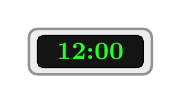
\begin{tikzpicture}\VeDongHoDienTu{0,0}{12:00}{gray}\end{tikzpicture}}
{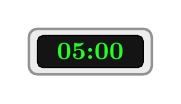
\begin{tikzpicture}\VeDongHoDienTu{0,0}{05:00}{gray}\end{tikzpicture}}
{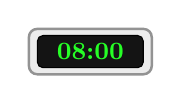
\begin{tikzpicture}\VeDongHoDienTu{0,0}{08:00}{gray}\end{tikzpicture}}
{\True 
\begin{tikzpicture}\VeDongHoDienTu{0,0}{04:00}{purple}\end{tikzpicture}}
\end{multicols}
\loigiai{
Kim ngắn chỉ số 4, kim dài chỉ số 12, biểu thị đúng 4 giờ. Đồng hồ điện tử tương ứng là \textbf{04:00}.\\
\textbf{Đáp án: D.}
}
\end{ex}

% CÂU 7: Tính thời gian làm việc ngoài đồng
\begin{ex} %[1H9H37]
Bác nông dân ra đồng làm việc từ 6 giờ sáng đến 9 giờ sáng:
\begin{center}\vspace{-2.5mm}
\begin{tikzpicture}
  \VeDongHoKim{0.55}{-2.2,0}{6}{myorange}
  \node[font=\bfseries\tiny, color=orange!90!black] at (-2.2,-0.85) {Bắt đầu: 6 giờ};
  \draw[->, >=stealth, line width=1.3pt, teal!90!black] (-0.8,0) -- (0.8,0) node[midway, above=2pt, font=\bfseries\tiny, color=black!85] {Thời gian làm việc};
  \VeDongHoKim{0.55}{2.2,0}{9}{myteal}
  \node[font=\bfseries\tiny, color=teal!90!black] at (2.2,-0.85) {Kết thúc: 9 giờ};
\end{tikzpicture}
\vspace{-2.5mm}\end{center}
Bác nông dân đã làm việc ngoài đồng trong khoảng thời gian bao lâu?
\begin{multicols}{4}
\choice
{$2$ giờ}
{$4$ giờ}
{\True $3$ giờ}
{$5$ giờ}
\end{multicols}
\loigiai{
Thời gian làm việc là: $9 - 6 = 3$ giờ.\\
\textbf{Đáp án: C.}
}
\end{ex}

% CÂU 8: Tính ngày tuần sau (+7 ngày)
\begin{ex} %[1H9V37]
Thứ Hai tuần này là ngày 6. Thứ Hai tuần sau là sinh nhật bạn Nam:
\begin{center}\vspace{-2.5mm}
\begin{tikzpicture}
  \VeToLich{-2.2,0}{THỨ HAI}{Ngày 6}{myblue}
  \draw[->, >=stealth, line width=1.3pt, red!85!black] (-0.8,0) -- (0.8,0) node[midway, above=2pt, font=\bfseries\tiny, color=blue!90!black] {Sau 1 tuần};
  \VeToLich{2.2,0}{THỨ HAI}{?}{myred}
\end{tikzpicture}
\vspace{-2.5mm}\end{center}
Sinh nhật bạn Nam vào ngày mấy của tháng đó?
\begin{multicols}{4}
\choice
{Ngày 12}
{Ngày 14}
{Ngày 15}
{\True Ngày 13}
\end{multicols}
\loigiai{
Sau 1 tuần lễ (7 ngày), Thứ Hai tuần sau sẽ là ngày: $6 + 7 = 13$.\\
\textbf{Đáp án: D.}
}
\end{ex}

\newpage
% --- TRANG 3: CÂU 9 ĐẾN CÂU 12 ---

% CÂU 9: Chuỗi hôm qua - hôm nay - ngày mai
\begin{ex} %[1H9V37]
Sơ đồ chuỗi ba ngày liên tiếp nhau:
\begin{center}\vspace{-2.5mm}
\begin{tikzpicture}[scale=0.85]
  \draw[fill=red!15, draw=red!80, line width=1pt, rounded corners=3pt] (-3.8,-0.5) rectangle (-1.8,0.5);
  \node[font=\bfseries\tiny, color=red!90!black] at (-2.8,0.18) {Hôm qua};
  \node[font=\bfseries\small, color=red!90!black] at (-2.8,-0.2) {Chủ nhật};

  \draw[->, >=stealth, line width=1.1pt, gray!80] (-1.7,0) -- (-1.1,0);

  \draw[fill=blue!15, draw=blue!80, line width=1pt, rounded corners=3pt] (-1.0,-0.5) rectangle (1.0,0.5);
  \node[font=\bfseries\tiny, color=blue!90!black] at (0,0.18) {Hôm nay};
  \node[font=\bfseries\small, color=blue!90!black] at (0,-0.2) {?};

  \draw[->, >=stealth, line width=1.1pt, gray!80] (1.1,0) -- (1.7,0);

  \draw[fill=teal!15, draw=teal!80, line width=1pt, rounded corners=3pt] (1.8,-0.5) rectangle (3.8,0.5);
  \node[font=\bfseries\tiny, color=teal!90!black] at (2.8,0.18) {Ngày mai};
  \node[font=\bfseries\small, color=teal!90!black] at (2.8,-0.2) {?};
\end{tikzpicture}
\vspace{-2.5mm}\end{center}
Nếu hôm qua là Chủ nhật thì ngày mai sẽ là thứ mấy?
\begin{multicols}{4}
\choice
{Thứ Hai}
{Thứ Tư}
{\True Thứ Ba}
{Thứ Bảy}
\end{multicols}
\loigiai{
Hôm qua là Chủ nhật $\implies$ Hôm nay là Thứ Hai $\implies$ Ngày mai là Thứ Ba.\\
\textbf{Đáp án: C.}
}
\end{ex}

% CÂU 10: Ca học buổi chiều
\begin{ex} %[1H9V37]
Lớp 1A học ca chiều từ 1 giờ chiều đến 4 giờ chiều:
\begin{center}\vspace{-2.5mm}
\begin{tikzpicture}
  \VeDongHoKim{0.55}{-2.2,0}{1}{myblue}
  \node[font=\bfseries\tiny, color=blue!90!black] at (-2.2,-0.85) {Bắt đầu: 1 giờ chiều};
  \draw[->, >=stealth, line width=1.3pt, orange!90!black] (-0.8,0) -- (0.8,0) node[midway, above=2pt, font=\bfseries\tiny, color=black!85] {Thời gian học};
  \VeDongHoKim{0.55}{2.2,0}{4}{myorange}
  \node[font=\bfseries\tiny, color=orange!90!black] at (2.2,-0.85) {Tan học: 4 giờ chiều};
\end{tikzpicture}
\vspace{-2.5mm}\end{center}
Lớp 1A học ca chiều trong khoảng thời gian bao lâu?
\begin{multicols}{4}
\choice
{$2$ giờ}
{\True $3$ giờ}
{$4$ giờ}
{$5$ giờ}
\end{multicols}
\loigiai{
Thời gian học là: $4 - 1 = 3$ giờ.\\
\textbf{Đáp án: B.}
}
\end{ex}

% CÂU 11: Chuyến du lịch cuối tuần
\begin{ex} %[1H9C37]
Dải các ngày trong kỳ nghỉ mát của gia đình bạn An:
\begin{center}\vspace{-2.5mm}
\begin{tikzpicture}[scale=0.68]
  \foreach \i/\thu/\mau in {1/{Thứ 5}/myblue, 2/{Thứ 6}/myblue, 3/{Thứ 7}/myorange, 4/{Chủ nhật}/myred} {
    \pgfmathsetmacro{\x}{(\i-2.5)*2.9}
    \draw[fill=\mau!20, draw=\mau!85, line width=1.1pt, rounded corners=3pt] (\x-1.05,-0.52) rectangle (\x+1.05,0.52);
    \node[font=\bfseries\footnotesize, color=\mau!90!black] at (\x,0) {\thu};
  }
\end{tikzpicture}
\vspace{-2.5mm}\end{center}
Gia đình An đi từ sáng Thứ Năm đến chiều Chủ nhật cùng tuần. Hỏi chuyến đi kéo dài mấy ngày?
\begin{multicols}{4}
\choice
{$3$ ngày}
{\True $4$ ngày}
{$5$ ngày}
{$6$ ngày}
\end{multicols}
\loigiai{
Chuyến đi gồm 4 ngày: Thứ Năm, Thứ Sáu, Thứ Bảy và Chủ nhật.\\
\textbf{Đáp án: B.}
}
\end{ex}

% CÂU 12: Thời gian sau 2 giờ buổi tối
\begin{ex} %[1H9V37]
Hiện tại đồng hồ đang chỉ 8 giờ tối:
\begin{center}\vspace{-2.5mm}
\begin{tikzpicture}
  \VeDongHoKim{0.55}{-2.2,0}{8}{mypurple}
  \node[font=\bfseries\tiny, color=purple!90!black] at (-2.2,-0.85) {Hiện tại: 8 giờ tối};
  \draw[->, >=stealth, line width=1.3pt, blue!85!black] (-0.8,0) -- (0.8,0) node[midway, above=2pt, font=\bfseries\tiny, color=black!85] {Sau 2 giờ nữa};
  \VeDongHoKim{0.55}{2.2,0}{10}{myblue}
  \node[font=\bfseries\tiny, color=blue!90!black] at (2.2,-0.85) {Sau 2 giờ: ?};
\end{tikzpicture}
\vspace{-2.5mm}\end{center}
Sau $2$ giờ nữa, đồng hồ sẽ chỉ mấy giờ tối?
\begin{multicols}{4}
\choice
{\True $10$ giờ tối}
{$9$ giờ tối}
{$11$ giờ tối}
{$12$ giờ đêm}
\end{multicols}
\loigiai{
Hiện tại là 8 giờ tối, sau 2 giờ nữa sẽ là: $8 + 2 = 10$ giờ tối.\\
\textbf{Đáp án: A.}
}
\end{ex}

\newpage
% --- TRANG 4: CÂU 13 ĐẾN CÂU 16 (ĐÚNG / SAI) ---

\textbf{Phần 2. Trắc nghiệm đúng sai}
\setcounterpageref{ex}{0}

% CÂU 13: Đặc điểm mặt đồng hồ
\begin{ex} %[1H9H37]
Quan sát chiếc đồng hồ treo tường đang chạy:
\begin{center}\vspace{-3mm}
\begin{tikzpicture}
  \VeDongHoKim{0.55}{0,0}{3}{myblue}
\end{tikzpicture}
\vspace{-3mm}\end{center}
Xét tính đúng hoặc sai của các khẳng định sau:
\choiceTF
{\True Kim ngắn dùng để chỉ giờ, kim dài dùng để chỉ phút.}
{\True Khi kim dài chỉ số 12 và kim ngắn chỉ số 3 thì đồng hồ chỉ 3 giờ đúng.}
{Một ngày đêm chỉ có tất cả 12 giờ.}
{\True Lúc 6 giờ đúng, kim ngắn và kim dài tạo thành một đường thẳng.}
\loigiai{\textbf{a)} Đúng. \textbf{b)} Đúng. \textbf{c)} Sai (Một ngày đêm có 24 giờ). \textbf{d)} Đúng (kim ngắn chỉ số 6, kim dài chỉ số 12 thẳng hàng).}
\end{ex}

% CÂU 14: Dải tuần lễ từ ngày 15 đến 21
\begin{ex} %[1H9V37]
Dải tuần lễ đi học và sinh hoạt từ ngày 15 đến ngày 21 của bạn Hà:
\begin{center}\vspace{-3mm}
\begin{tikzpicture}
  \VeDaiTuanCoNgay{0,0}{15}
\end{tikzpicture}
\vspace{-3mm}\end{center}
Xét tính đúng hoặc sai của các khẳng định sau:
\choiceTF
{\True Thứ Hai là ngày 15 và Chủ nhật là ngày 21.}
{Thứ Tư là ngày 18.}
{\True Thứ Bảy (ngày 20) và Chủ nhật (ngày 21) là hai ngày nghỉ cuối tuần.}
{\True Trong tuần lễ đó bạn Hà đi học 5 ngày (từ Thứ Hai đến Thứ Sáu).}
\loigiai{\textbf{a)} Đúng. \textbf{b)} Sai (Thứ Tư là ngày 17, ngày 18 là Thứ Năm). \textbf{c)} Đúng. \textbf{d)} Đúng (5 ngày: 15, 16, 17, 18, 19).}
\end{ex}

% CÂU 15: Lịch trình Chủ nhật của Bình
\begin{ex} %[1H9V37]
Các mốc thời gian hoạt động ngày Chủ nhật của Bình:
\begin{center}\vspace{-3mm}
\begin{tikzpicture}
  \VeDongHoKim{0.45}{-3.4,0}{7}{myteal}
  \node[font=\bfseries\tiny, color=teal!90!black] at (-3.4,-0.7) {7h: Dậy};
  \VeDongHoKim{0.45}{-1.15,0}{10}{myorange}
  \node[font=\bfseries\tiny, color=orange!90!black] at (-1.15,-0.7) {10h: Vẽ};
  \VeDongHoKim{0.45}{1.15,0}{3}{myblue}
  \node[font=\bfseries\tiny, color=blue!90!black] at (1.15,-0.7) {3h: Bóng};
  \VeDongHoKim{0.45}{3.4,0}{7}{mypurple}
  \node[font=\bfseries\tiny, color=purple!90!black] at (3.4,-0.7) {7h: Cơm};
\end{tikzpicture}
\vspace{-3mm}\end{center}
Xét tính đúng hoặc sai của các khẳng định sau:
\choiceTF
{\True Bình thức dậy tập thể dục lúc 7 giờ sáng.}
{Bình học vẽ tranh lúc 11 giờ trưa.}
{\True Bình đi đá bóng cùng các bạn lúc 3 giờ chiều.}
{\True Khoảng cách thời gian từ lúc đá bóng (3h chiều) đến lúc ăn cơm tối (7h tối) là 4 giờ.}
\loigiai{\textbf{a)} Đúng. \textbf{b)} Sai (Bình học vẽ lúc 10 giờ sáng). \textbf{c)} Đúng. \textbf{d)} Đúng ($7 - 3 = 4$ giờ).}
\end{ex}

% CÂU 16: Nhận định về lịch tuần và ngày tháng
\begin{ex} %[1H9H37]
Quan sát hai tờ lịch Thứ Năm của hai tuần liên tiếp:
\begin{center}\vspace{-3mm}
\begin{tikzpicture}
  \VeToLich{-1.8,0}{THỨ NĂM}{Ngày 8}{myblue}
  \VeToLich{1.8,0}{THỨ NĂM}{Ngày 15}{myteal}
\end{tikzpicture}
\vspace{-3mm}\end{center}
Xét tính đúng hoặc sai của các khẳng định sau:
\choiceTF
{\True Thứ Năm tuần sau cách Thứ Năm tuần trước đúng 7 ngày.}
{\True Nếu ngày 8 là Thứ Năm thì ngày 15 cũng là Thứ Năm vì $8 + 7 = 15$.}
{Ngày liền trước ngày 8 là ngày 9.}
{Trong một tuần lễ, ngày liền sau ngày Thứ Bảy là ngày Thứ Hai.}
\loigiai{\textbf{a)} Đúng. \textbf{b)} Đúng. \textbf{c)} Sai (Ngày liền trước ngày 8 là ngày 7). \textbf{d)} Sai (Ngày liền sau Thứ Bảy là Chủ nhật).}
\end{ex}

\newpage
% --- TRANG 5: CÂU 17 ĐẾN CÂU 20 (TRẢ LỜI NGẮN) ---

\textbf{Phần 3. Trả lời ngắn}
\setcounterpageref{ex}{0}

% CÂU 17: Đọc giờ đi ngủ buổi tối
\begin{ex} %[1H9N37]
Buổi tối, bạn Mai bắt đầu đi ngủ khi đồng hồ treo trong phòng chỉ như hình vẽ:
\begin{center}\vspace{-2.5mm}
\begin{tikzpicture}
  \VeDongHoKim{0.65}{0,0}{9}{mypurple}
\end{tikzpicture}
\vspace{-2.5mm}\end{center}
Hỏi bạn Mai đi ngủ lúc mấy giờ tối?
\shortans{9}
\loigiai{
Kim ngắn chỉ số 9, kim dài chỉ số 12. Vậy Mai đi ngủ lúc 9 giờ tối.\\
\textbf{Đáp số:} $9$.
}
\end{ex}

% CÂU 18: Tính thời gian xem phim hoạt hình
\begin{ex} %[1H9H37]
Bộ phim hoạt hình chiếu từ 7 giờ tối đến 9 giờ tối:
\begin{center}\vspace{-2.5mm}
\begin{tikzpicture}
  \VeDongHoKim{0.55}{-2.2,0}{7}{myblue}
  \node[font=\bfseries\tiny, color=blue!90!black] at (-2.2,-0.85) {Bắt đầu: 7 giờ tối};
  \draw[->, >=stealth, line width=1.3pt, orange!90!black] (-0.8,0) -- (0.8,0) node[midway, above=2pt, font=\bfseries\tiny, color=black!85] {Thời lượng phim};
  \VeDongHoKim{0.55}{2.2,0}{9}{myorange}
  \node[font=\bfseries\tiny, color=orange!90!black] at (2.2,-0.85) {Kết thúc: 9 giờ tối};
\end{tikzpicture}
\vspace{-2.5mm}\end{center}
Hỏi bộ phim hoạt hình đó kéo dài trong mấy giờ?
\shortans{2}
\loigiai{
Thời lượng bộ phim là: $9 - 7 = 2$ giờ.\\
\textbf{Đáp số:} $2$.
}
\end{ex}

% CÂU 19: Tính ngày theo tuần lễ lùi 1 tuần (-7 ngày)
\begin{ex} %[1H9V37]
Thứ Tư tuần này là ngày 18 tháng 3:
\begin{center}\vspace{-2.5mm}
\begin{tikzpicture}
  \VeToLich{-2.2,0}{THỨ TƯ}{?}{myteal}
  \draw[->, >=stealth, line width=1.3pt, purple!90!black] (-0.8,0) -- (0.8,0) node[midway, above=2pt, font=\bfseries\tiny, color=blue!90!black] {Tuần sau};
  \VeToLich{2.2,0}{THỨ TƯ}{Ngày 18}{myblue}
\end{tikzpicture}
\vspace{-2.5mm}\end{center}
Hỏi Thứ Tư tuần trước đó là ngày bao nhiêu của tháng 3?
\shortans{11}
\loigiai{
Thứ Tư tuần trước cách 1 tuần (7 ngày) trước: $18 - 7 = 11$. Vậy là ngày 11 tháng 3.\\
\textbf{Đáp số:} $11$.
}
\end{ex}

% CÂU 20: Tính ngày tiến 1 tuần (+7 ngày)
\begin{ex} %[1H9V37]
Ngày 20 tháng 10 là ngày Thứ Hai. Hội diễn văn nghệ của trường sẽ diễn ra vào Thứ Hai tuần sau:
\begin{center}\vspace{-2.5mm}
\begin{tikzpicture}
  \VeToLich{-2.2,0}{THỨ HAI}{Ngày 20}{myorange}
  \draw[->, >=stealth, line width=1.3pt, teal!90!black] (-0.8,0) -- (0.8,0) node[midway, above=2pt, font=\bfseries\tiny, color=blue!90!black] {Sau 1 tuần};
  \VeToLich{2.2,0}{THỨ HAI}{?}{myred}
\end{tikzpicture}
\vspace{-2.5mm}\end{center}
Hỏi hội diễn văn nghệ diễn ra vào ngày bao nhiêu tháng 10?
\shortans{27}
\loigiai{
Sau 1 tuần lễ (7 ngày), Thứ Hai tuần sau sẽ là ngày: $20 + 7 = 27$ tháng 10.\\
\textbf{Đáp số:} $27$.
}
\end{ex}
